%\part{Konstruktion}
%\chapter{Programmlogik}
%\section{QueryResolution}

\subsection{QueryBuild}

\begin{figure}[htb]
	\centering
  	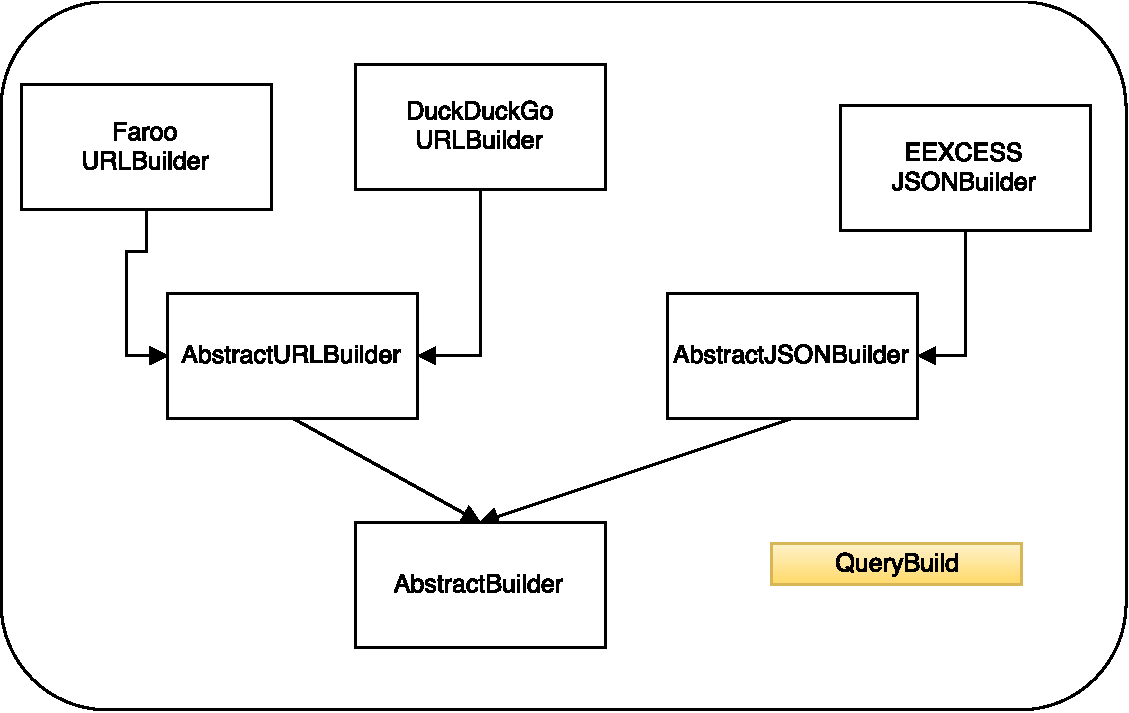
\includegraphics[width=\textwidth]{qr_querybuild}
  	\caption{Aufbau des Moduls \lstinline|QueryBuild|}
\end{figure}

Das Modul \lstinline|QueryBuild| liefert Hauptintelligenz im Modul \lstinline|QueryResolution|. Seine Aufgaben sind es, die \lstinline|ConnectionController| in \lstinline|QuerySend| zu konfigurieren, die Query in das suchmaschinenspezifische Anfrageformat umzuwandeln und anschließend dem \lstinline|ConnectionController| den Parser für die Antwort zu geben.

Jede Suchmaschine hat eine Implementierung der Spezifikation \lstinline|AbstractBuilder|, welche durch \lstinline|URLAbstractBuilder| und \lstinline|JSONAbstractBuilder| erweitert wird.